\section{Train/Test Data Extraction}

\subsection{Ground Truth Glyph Examples}

The ground truth data provided by the contest contained image files, each with multiple bounding boxes and glyphs. To extract this data for the purposes of training and evaluation of classification and bounding methods, each original image was copied and cropped to contain only one glyph, generating a single cropped image, cut to the exact bounding box given, for each glyph \seefig{cropped_ground_truth_glyphs}. To extract the isolated glyph images for training, the following method is used. For each image in the training data, the image was loaded, and the COCO file provided by the contest was utilized to find each annotated glyph. For each glyph, the loaded image was duplicated and cropped to the bounding box provided in the COCO file. The cropped image was then saved to file either separated by glyph class, or without any class label.
Each cropped glyph file was saved with information on which image the glyph was cropped from, the style it was written in \seefig{xi_footmarktype}, and the preservation of the glyph \seefig{omega_basetype}.

These methods were used to extract glyph images from both the binarized images and un-altered images. Similar processes were also used to generate training data for the various CNNs, and external tools utilized in the project.

\begin{figure}
    \caption{Ground Truth Glyph Examples}
    \label{fig:cropped_ground_truth_glyphs}
    \begin{center}
    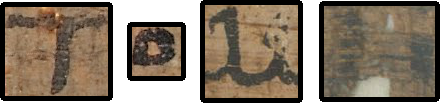
\includegraphics[width=0.75\textwidth]{{glyphs/cropped_ground_truth_glyphs.png}}
    \end{center}
    Four examples of the bounded glyphs provided by the contest training data. All the glyphs provided in the training and test data are uppercase and bounded by hand-drawn bounding boxes, which appear here. The first glyph, a $\Gamma$, is well formed, but has the noise from another glyph on the left side and is truncated by the bounding box on the right side. Similarly, the second glyph, an $A$, is well formed, but has the noise from another glyph on the left side and is truncated by the bounding box on the right and bottom sides. The third glyph, an $I$, is not cut off, but does have a line from a neighboring glyph as well. It also shows the edge of the papyrus. The fourth glyph, another $A$, is an example of the varying image quality of the training data, showing obvious artifacting or distortion.
\end{figure}

\begin{figure}
    \caption{Styles of $\Xi$ in the Training Data}
    \label{fig:xi_footmarktype}
    \begin{center}
    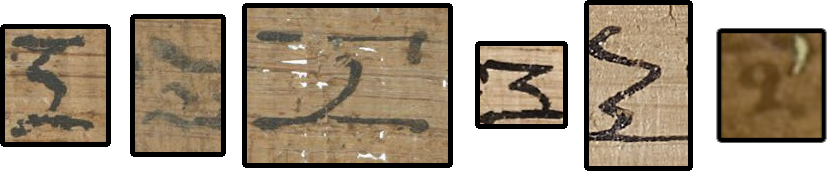
\includegraphics[width=0.75\textwidth]{{glyphs/xi_footmarktype.png}}
    \end{center}
    Examples of the six unique styles for the letter $\Xi$, as determined by the authors of the contest this project was based on. Numbered from 1-6 left to right. The furthest right image of a $\Xi$ was resized for the purpose of display in the figure, which has increased the blurriness of the image.
\end{figure}

\begin{figure}
    \caption{Examples of Preservation Levels in $\Omega$'s in Training Data}
    \label{fig:omega_basetype}
    \begin{center}
    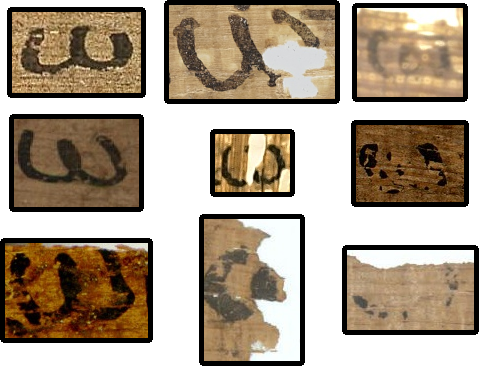
\includegraphics[width=0.75\textwidth]{{glyphs/omega_basetype.png}}
    \end{center}
    Examples of the three levels of preservation for the letter $\Omega$ (appearing as the unical manuscript form, which looks similar to a larger lowercase modern $\omega$), as determined by the authors of the contest this project was based on. Numbered from 1-3 left to right. There are three examples of each level to display three examples of the various degradations that lead to being in each level. The least degraded level (1) is defined as a complete or nearly complete glyph. The second least degraded level (2) is defined as an incomplete letter that unambiguously belongs to one class. The most degraded level in the dataset (3), requires context to determine its actual class, as the glyph may appear to potentially be one of multiple classes when viewed in isolation.
\end{figure}

\subsection{Tightly Bound Glyph Examples}
\todo{TODO}

\subsection{Greek Language Corpus}

To form the training data for a language model, the entirety of the Greek section of the Perseus Digital Library \cite{Perseus} dataset was downloaded. The data was converted from XML to plain text and cleaned of all non-standard Greek letters utilizing a mix of regex, python string functions and a list of the glyphs that appear in the training set of images. When removing invalid characters, the passages that they appeared in were also removed to ensure the integrity of the training data. To ensure the language data was as close to the image training data as possible, all diacritics and punctuation marks were removed, and the letters were converted to their uppercase variant. The remaining data contains $~46,400,000$ glyphs. This data was used to generate five smaller files for the purposes of training language models by randomly selecting chunks from the data.


\section{Binarization}
\todo{NEW}

A perfect binarized version of a papyrus image is defined by a background color and ink color, where the ink is black, and the background is white. Each pixel in an image is altered so that it is either black or white, depending on if it is ink or anything else (background). As no ground truth for ink was given to train on, all the methods for binarization are based on either pre-trained CNNs or algorithmic solutions utilized in similar problems.

\subsection{Clustering}
\todo{NEW}

Clustering based binarization is performed with k-means clustering. For each image, the pixels of the image were placed in a 3d space with their red, green, and blue values being used to determine their location. Pixels were then clustered in groups using k-means clustering. The pixel cluster which contained the value closest to black was then utilized as the ink cluster, with all pixels not in that cluster being labeled as the background.

\subsection{Filtering}
\todo{NEW}

Filtering based binarizations are generated utilizing the Gabor filtering  \cite{Gabor1949, Gabor1948} to find clusters of pixels that are not like those around them, which could be glyphs. Gabor filtering is based on a linear filter, but when multiple linear filters are grouped together with a set rotation applied to each subsequent filter, a 2d filter can be generated to generate a simplification of Gabor wavelets \cite{Gabor1949, Gabor1948}. Using these 2d filters, this method of binarization seeks to find features in an image that has a specific frequency, which in the case of glyphs might be the width or height of a single line in a glyph.

This method requires an assumption on the wave frequency that may generate the glyphs, so a manual heuristic method was utilized to generate the function that most accurately generated the correct wave for the images in the training dataset.

\subsection{Input Invarient Thresholding}
\todo{TODO}

\subsection{DP-Linknet}
\todo{TODO}

\subsection{BiNet}
\todo{TODO}


\section{Glyph Bounding}

\subsection{Bounding Boxes}
\todo{TODO}

\subsection{Connected Components}
\todo{TODO}

\subsection{Sliding Window Region Based Convolution Neural Networks}
\todo{TODO}


\section{Line Bounding}

\subsection{Point Of Interest Clustering}
\todo{DOG + POI + adaptive dbscan}

\subsection{Point Of Interest Clustering}
\todo{TODO}

\subsection{Adjacent Glyph Clustering}
\todo{TODO}

\subsection{Overlaping Glyph Clustering}
\todo{TODO}


\section{Classification}

\subsection{Transfer Learning}
\todo{TODO}

\subsection{Convolutional Neural Networks}
\todo{TODO}

\subsection{Stochastic Language Models}
\todo{TODO}

\subsection{Neural Netork Language Models}
\todo{TODO}


\section{Existing Pipelines}

For the sake of completeness, Tesseract \cite{SmithTesseract}, a popular OCR engine sponsored by Google \cite{Vincent} and Ocular, another OCR engine based on Stochastic models were integrated into the pipeline using pytesseract \cite{Lee} and by calling jar files from python respectively.
